\documentclass[10pt,a4paper]{article}

\usepackage{datetime}
\usepackage{numprint}
\usepackage{palatino}
\usepackage{authblk}
\usepackage[margin=0.75in]{geometry}
\usepackage{hyperref}
\usepackage{graphicx}
\usepackage{titlesec}
\usepackage{listings}
\usepackage[english]{babel}
\usepackage[
	backend=biber,
	style=numeric,
]{biblatex}
\addbibresource{refs.bib}

\hypersetup{%
    pdfborder = {0 0 0}
}

\setlength{\parindent}{2em}
%\setlength{\parskip}{1em}
\renewcommand{\baselinestretch}{1.0}

\begin{document}

\nplpadding{2}

\title{Malware Analysis Report: ``Practical1.exe''\\ \vspace{-8pt} {\large CAP6137 Malware Reverse Engineering: P0x01}}
\author{{Naman Arora \\ \vspace{-10pt}\small \href{mailto:naman.arora@ufl.edu}{naman.arora@ufl.edu}}}
\date{\today}

\maketitle
\newpage
\tableofcontents
\newpage
\section{Executive Summary}
The acquired malware binary is a very sophisticated malware sample. It possibly is from the malware family \textit{Carberp} from 2009 and has possible functionalities of mass infection like BotNets, keylogging, browser User agents, and banking data exfiltration. The malware, on execution, copies itself to a location where it gains persistance over reboots. It injects itself to benign services memory regions in \textit{Windows Kernel Space}. Statically analyzing the sample does not lead to much gains so dynamic analysis is more fruitful. It exhibits a very effective obfuscation behavior possibly via code compression which it de-compresses at run time. Other obfuscation methods come into play when it tries to exfiltrate gathered information to its \textit{C2}. All of the information sent is possibly encrypted.

On execution, it decompresses itself, copies itself for persistance and starts a \textit{`svchost'} process where it injects itself. The parent process exists resulting an unlinked \textit{`svchost'} process. The malware then possibly hooks into keylogging API and listens for other as of yet unidentified events. After event logging, it sends back the information via HTTP POST API to its \textit{C2}.

\section{Static Analysis}
\subsection{Basic Identification}
The provided malware binary sample has the following information in the binary,
\begin{center}
	\begin{tabular}{c | c}
		Attribute & Value\\
		\hline
		\hline
		Bits & 32\\
		Endianess & Little\\
		Operating System & Microsoft Windows\\
		\hline
		Class & Portable Executable (PE)\\
		Subsystem & Microsoft Windows GUI\\
		\hline
		Size & 157184 bytes\\
		Compiler Timestamp & Wed, Nov 19, 2008, 20:24:19\\
		Debugger Timestamp & Sun, June 19, 2011, 17:31:54\\
		SHA256 Hash & a67a1ca66f666eabef466bd6beba25867fd67ba697c1c7c02cde2c51e4e8289d\\
		\hline
	\end{tabular}
\end{center}

\subsection{Malware Sample Family Identification}
\begin{figure}[!htbp]% [!hb] forces image to be placed at that position
	\centering
	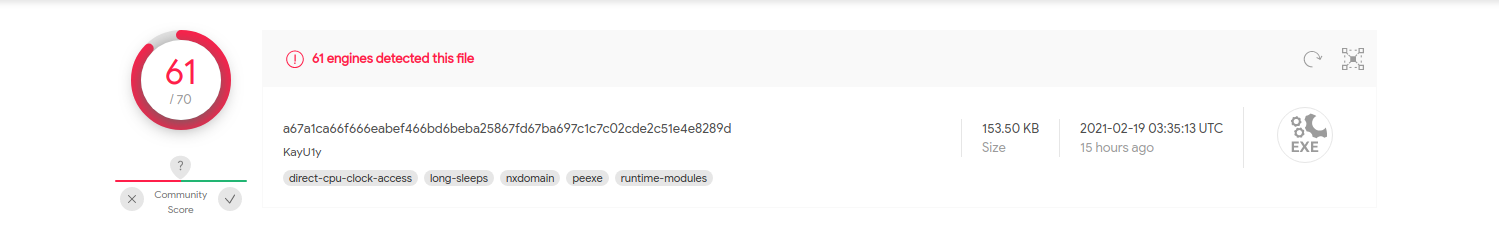
\includegraphics[width=\columnwidth]{pics/virustotal.png}
	\caption{Virustotal Detection}
	\label{Virustotal}
\end{figure}
When searched using the SHA256 hash of the sample on \textit{www.virustotal.com} for any prior detections,
an overwhelming majority of services detect the sample as malicious executable, \textit{61/70} to be exact.
The sample is linked to \textit{Carberp} \cite{carberp} family of trojans which was infamous for attacking banking systems during 2009.

\subsection{PE Sections}
The PE has \textbf{\textit{five identifiable}} sections (Fig. \ref{rizin_sections}).
\begin{figure}[!htbp]% [!hb] forces image to be placed at that position
	\centering
	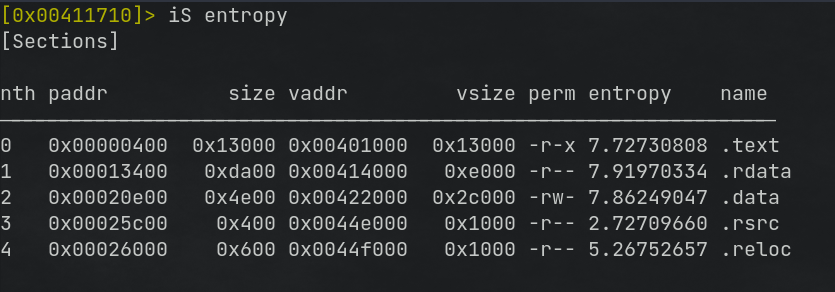
\includegraphics[width=\columnwidth]{pics/rizin_section.png}
	\caption{Rizin: PE Sections with Entropy}
	\label{rizin_sections}
\end{figure}

	\subsubsection{The Text section}
		The text section is supposed to contain the executable code within a binary.
		While the given binary shows expected permissions of Read and Execute,
		it shows an unusually high entropy of 7.72 which should be noted and will be referenced in later sections.
		The size and virtual size of the section are exactly the same, \textit{i.e., 0x13000}.

	\subsubsection{The Rdata Section}
		The Rdata section contains read only data which the binary needs.
		This could be global constants and read only data.
		The Rdata section too shows unusually high entropy of 7.91 which hints more towards compressed or encrypted data.
		The virtual size of this section \textit{0xe000} is slightly larger than static size \textit{0xda00} which is common.
		Permissions on this section are as expected, \textit{i.e.}, Read only.

	\subsubsection{The Data Section}
		The data section contains writable data for the binary. The permissions on this section, too, are as expected.
		This section too shows an unusually high entropy of 7.86.
		Moreover, the virtual size of this section is around 8x times more than the static size, which is very unusual.
		Overall, this hints towards compressed data.

	\subsubsection{The Resource and Re-allocation Sections}
		Both of these sections have a virtual size of \textit{0x1000} with static sizes of \textit{0x400} and \textit{0x600} respectively.
		The entropies and the size inflation is not too out of the ordinary.

\subsection{A case for Compression}
The given malware section exhibits unusually high entropy for the first four sections.
Generally, such a high entropy is associated with either of the three obfuscation techniques \textit{viz.}
Compression, Encryption or Packing.
Given the static analysis, packing can be eliminated with relatively high degree of confidence since the binary also
shows a multitude of embedded strings, library calls and imports.
As for encryption versus compression, three imports, in particular, indicate usage of LZMA \cite{lzma} compression algorithm (Fig. \ref{lzma}).
Moreover, an 8x inflation in size of the \textit{.data} section, as mentioned above, too indicates such a possibility.
\begin{figure}[!htbp]% [!hb] forces image to be placed at that position
	\centering
	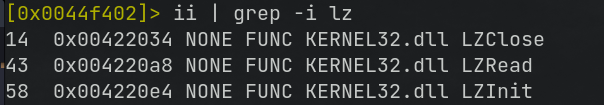
\includegraphics[width=\columnwidth]{pics/lzma.png}
	\caption{Rizin: Imports from lzexpand.h}
	\label{lzma}
\end{figure}

\subsection{Interesting Imports}
	\subsubsection{WS2\_32 and Berkley Socket API}
		\begin{figure}[!htbp]% [!hb] forces image to be placed at that position
			\centering
			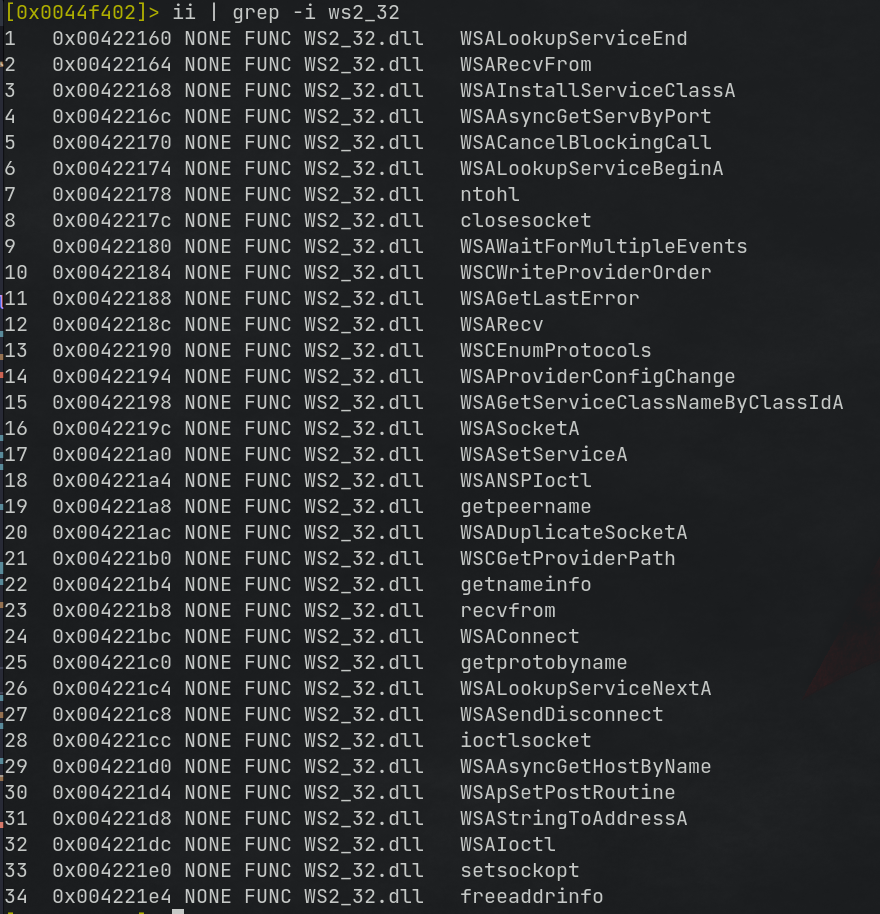
\includegraphics[width=\columnwidth]{pics/ws2_32.png}
			\caption{Rizin: Imports WS2\_32.dll}
			\label{ws2_32}
		\end{figure}
		Imports such as \textit{ntohl, closesocket, setsockopt, recvfrom, getpeername, etc.} strongly indicate
		an internet based socket activity.
		Also, the presence of other imports from WS2\_32.dll, indicate a strong presence of UDP/connectionless protocol.
		This could be due to the application querying DNS records.

	\subsubsection{Wininet API}
		\begin{figure}[!htbp]% [!hb] forces image to be placed at that position
			\centering
			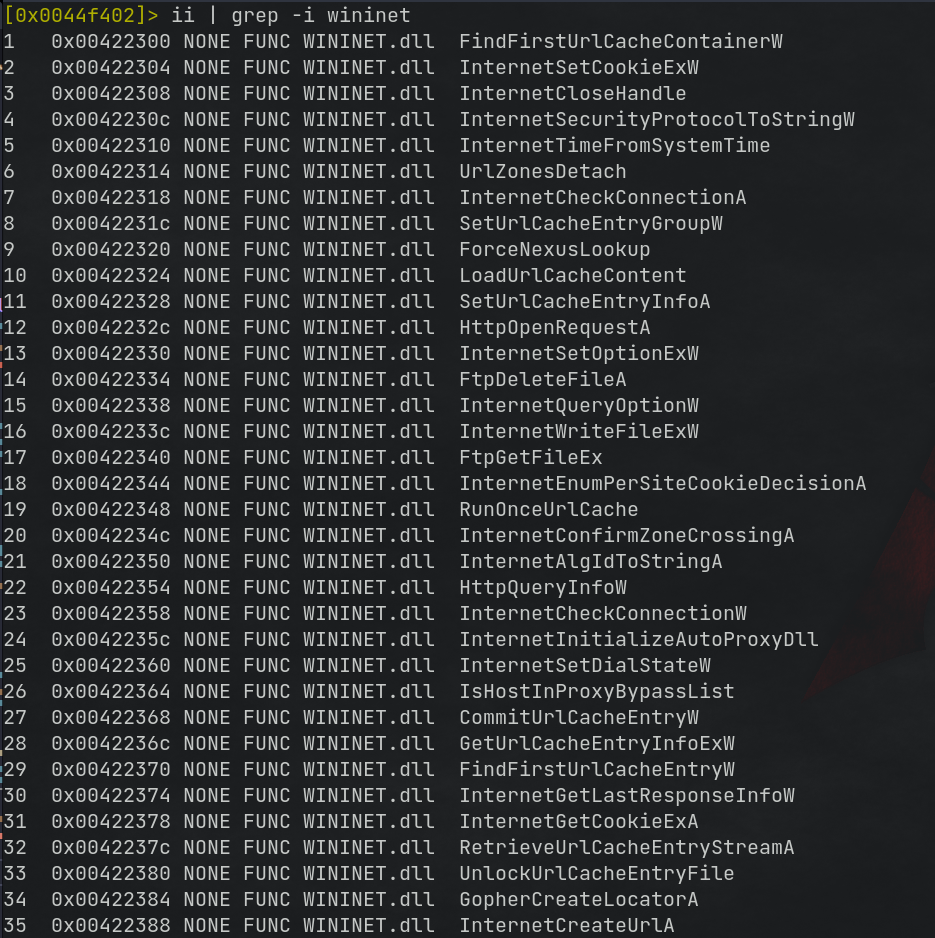
\includegraphics[width=\columnwidth]{pics/wininet.png}
			\caption{Rizin: Imports Wininet.dll}
			\label{wininet}
		\end{figure}
		\begin{itemize}
			\item{HTTP}\\
				Imports such as \textit{HttpQueryInfo, HttpOpenRequest, etc.} strongly indicate towards HTTP related activity.
			\item{FTP}\\
				Imports such as \textit{FtpGetFileEx, FtpDeleteFileA, etc.} strongly indicate towards read and write activity
				to a remote server over FTP protocol.
			\item{Browser Related Activity}\\
				Imports such as \textit{InternetSetCookieExW, LoadUrlCacheContent, etc.} suggest some interaction with browser
				cache.
		\end{itemize}
		Even though these imports strongly suggest their mentioned intentions, no strings that point to any remote address
		have been located in the binary statically. This makes the case for compression based obfuscation stronger.

	\subsubsection{Other Miscallineous Imports}
		\begin{figure}[!htbp]% [!hb] forces image to be placed at that position
			\centering
			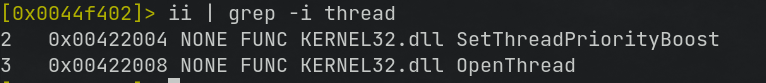
\includegraphics[width=\columnwidth]{pics/impThr.png}
			\caption{Rizin: Imports Threading}
			\label{impThr}
		\end{figure}
		\begin{figure}[!htbp]% [!hb] forces image to be placed at that position
			\centering
			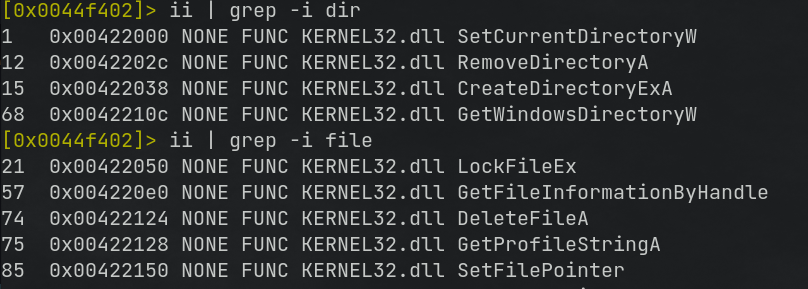
\includegraphics[width=\columnwidth]{pics/impFile.png}
			\caption{Rizin: Imports File System}
			\label{impFile}
		\end{figure}
		Other interesting imports,
		\begin{itemize}
			\item Threading functionality (Fig. \ref{impThr})
			\item File System related functionality (Fig. \ref{impFile})
		\end{itemize}

\section{Dynamic Analysis}
		\subsection{Network Based Analysis}
			\subsubsection{External domains contacted}
				\begin{figure}[!htbp]% [!hb] forces image to be placed at that position
					\centering
					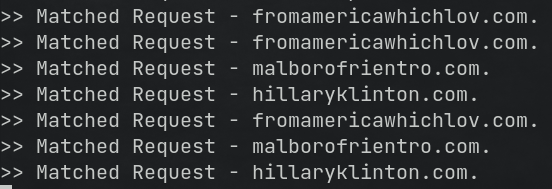
\includegraphics[width=\columnwidth]{pics/fakedns.png}
					\caption{FakeDNS: DNS Domain Lookups}
					\label{fakedns}
				\end{figure}
				The malware attempts to make a connection to the following domains(Fig. \ref{fakedns}),
				\begin{itemize}
					\item fromamericawhichlove.com
					\item hillaryklinton.com
					\item malborofrientro.com
				\end{itemize}
			\subsubsection{Internet Protocols Used}
				\begin{figure}[!htbp]% [!hb] forces image to be placed at that position
					\centering
					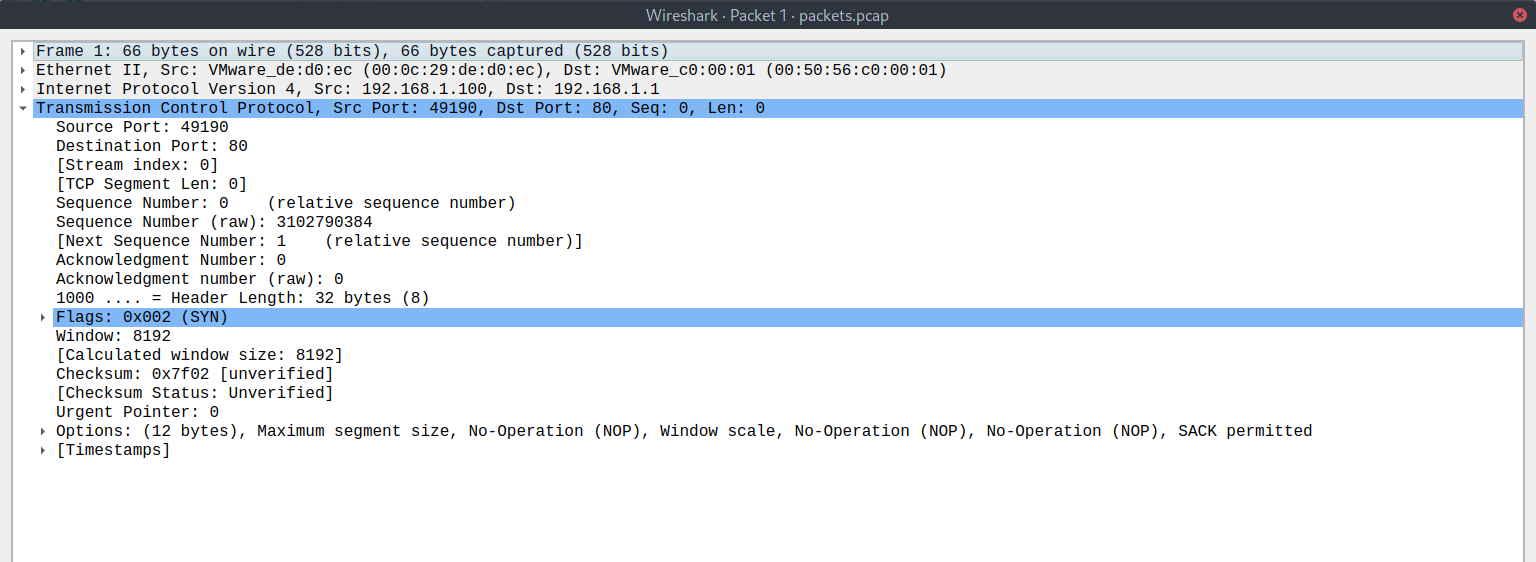
\includegraphics[width=\columnwidth]{pics/tcpsyn.png}
					\caption{Wireshark: TCP SYN request}
					\label{tcpsyn}
				\end{figure}
				\begin{figure}[!htbp]% [!hb] forces image to be placed at that position
					\centering
					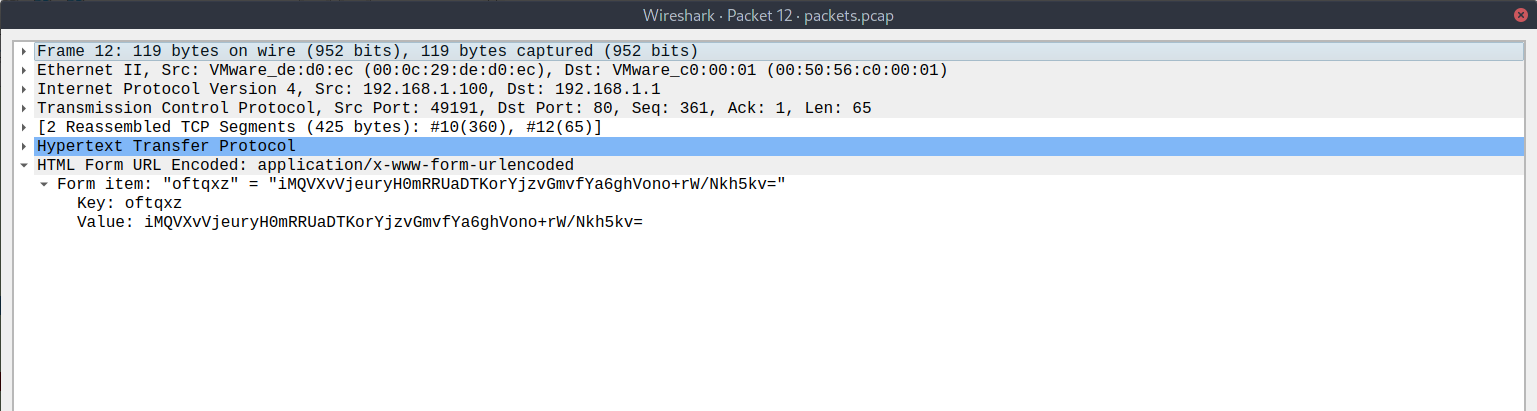
\includegraphics[width=\columnwidth]{pics/httppost.png}
					\caption{Wireshark: HTTP Post with Base64 Encoded value}
					\label{httppost}
				\end{figure}
				The malware on execution uses the following Protocols
				\begin{itemize}
					\item DNS over UDP\\
						The malware queries for hosts using DNS lookup.
						The DNS server used is the same as the default on the host system.
					\item HTTP POST over TCP\\
						The malware sends multiple POST requests (every 60sec or so) containing base64 encoded files.
						The files can have extensions \textit{.phtml, .php3, .phtm, .inc, .cgi, .doc, .rtf, .tpl and .rar}.
						The list of extensions will be proved using memory forensics.
				\end{itemize}
			\subsubsection{Contents of Communication}
				The malware communicates information over the internet to previously specified domains using HTTP POST
				requests. The communication contains a file with key value pair.
				The \textit{key} is seemingly random while the \textit{value} happens to be a Base64 encoded string.
				On decoding the \textit{value}, a seemingly encrypted sequence of bytes is obtained.

		\subsection{File System Based Analysis}
				\begin{figure}[!htbp]% [!hb] forces image to be placed at that position
					\centering
					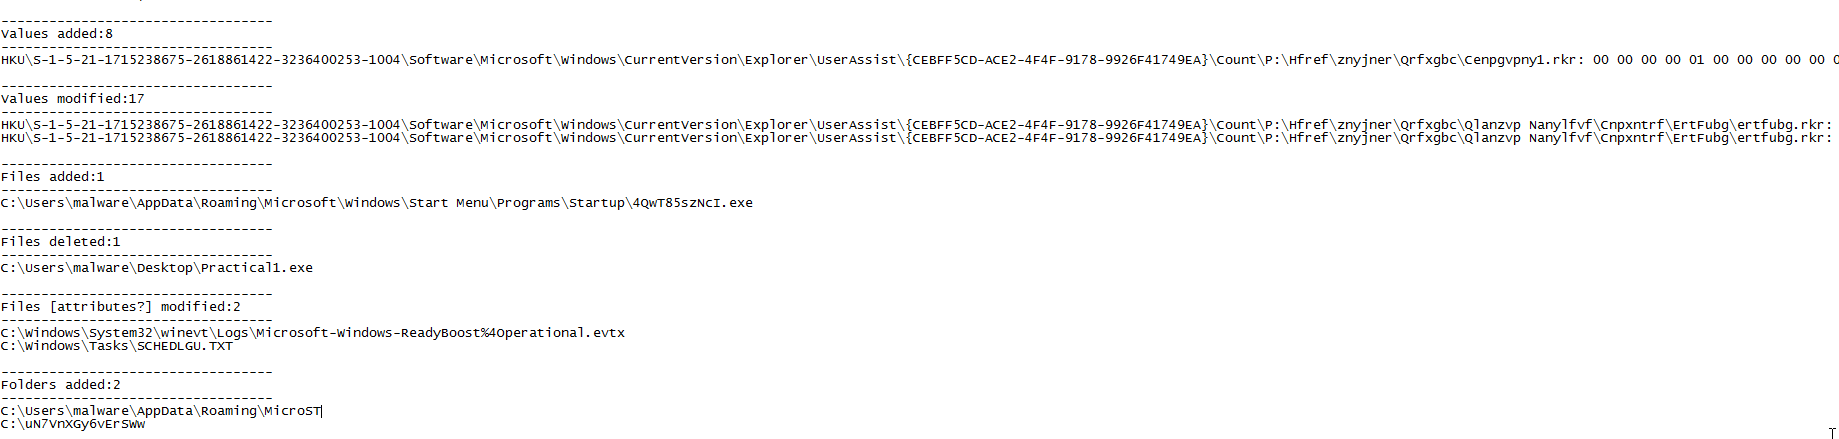
\includegraphics[width=\columnwidth]{pics/regshot.png}
					\caption{RegShot: File system Changes}
					\label{regshot}
				\end{figure}
				\subsubsection{File System Changes}
					\begin{figure}[!htbp]% [!hb] forces image to be placed at that position
						\centering
						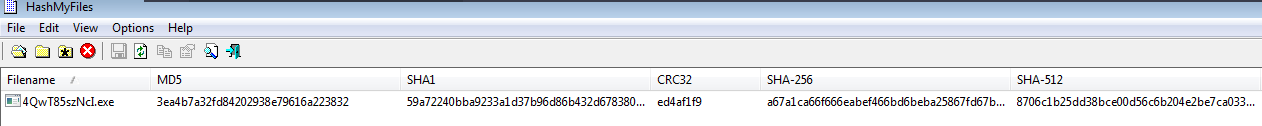
\includegraphics[width=\columnwidth]{pics/dropped.png}
						\caption{HashMyFiles: Hash of dropped file}
						\label{dropped}
					\end{figure}
					The copy of the binary which is executed at first instantiation is deleted.
					The malware then achieves persistance by copying itself to the location
					\textit{``\%USERPROFILE\%\textbackslash AppData\textbackslash Roaming\textbackslash Microsoft\textbackslash Windows\textbackslash Start Menu\textbackslash Programs\textbackslash Startup\textbackslash 4QwT85szNcI.exe''}
					The dropped file has the same hash as the original file (Fig. \ref{dropped}).

					The malware creates two directories, \textit{viz.}
					\begin{itemize}
						\item \textit{``\%USERPROFILE\%\textbackslash AppData\textbackslash Roaming\textbackslash MicroST''}
						\item \textit{``C:\textbackslash uN7vnXGy6vErSWw''}
					\end{itemize}

				\subsubsection{Windows Registry Changes}
					The malware changes the registry key,\\
						\textit{``HKU\textbackslash S-1-5-21-1715238675-2618861422-3236400253-1004\textbackslash Software\textbackslash Microsoft\textbackslash Windows\textbackslash CurrentVersion\textbackslash Explorer\textbackslash UserAssist\textbackslash\{CEBFF5CD-ACE2-4F4F-9178-9926F41749EA\}\textbackslash Count\textbackslash P:\textbackslash Hfref\textbackslash znyjner\textbackslash Qrfxgbc\textbackslash Qlanzvp Nanylfvf\textbackslash Cnpxntrf\textbackslash ErtFubg\textbackslash ertfubg.rkr''}


					The malware creates a registry key,\\
						\textit{``HKU\textbackslash S-1-5-21-1715238675-2618861422-3236400253-1004\textbackslash Software\textbackslash Microsoft\textbackslash Windows\textbackslash CurrentVersion\textbackslash Explorer\textbackslash UserAssist\textbackslash\{CEBFF5CD-ACE2-4F4F-9178-9926F41749EA\}\textbackslash Count\textbackslash P:\textbackslash Hfref\textbackslash znyjner\textbackslash Qrfxgbc\textbackslash Cenpgvpny1.rkr''}

		\subsection{Memory Forensics}
				The memory of a running Virtual Machine infected with the malware was dumped and analyzed.
				\subsubsection{The malicious memory regions}
					\begin{figure}[!htbp]% [!hb] forces image to be placed at that position
						\centering
						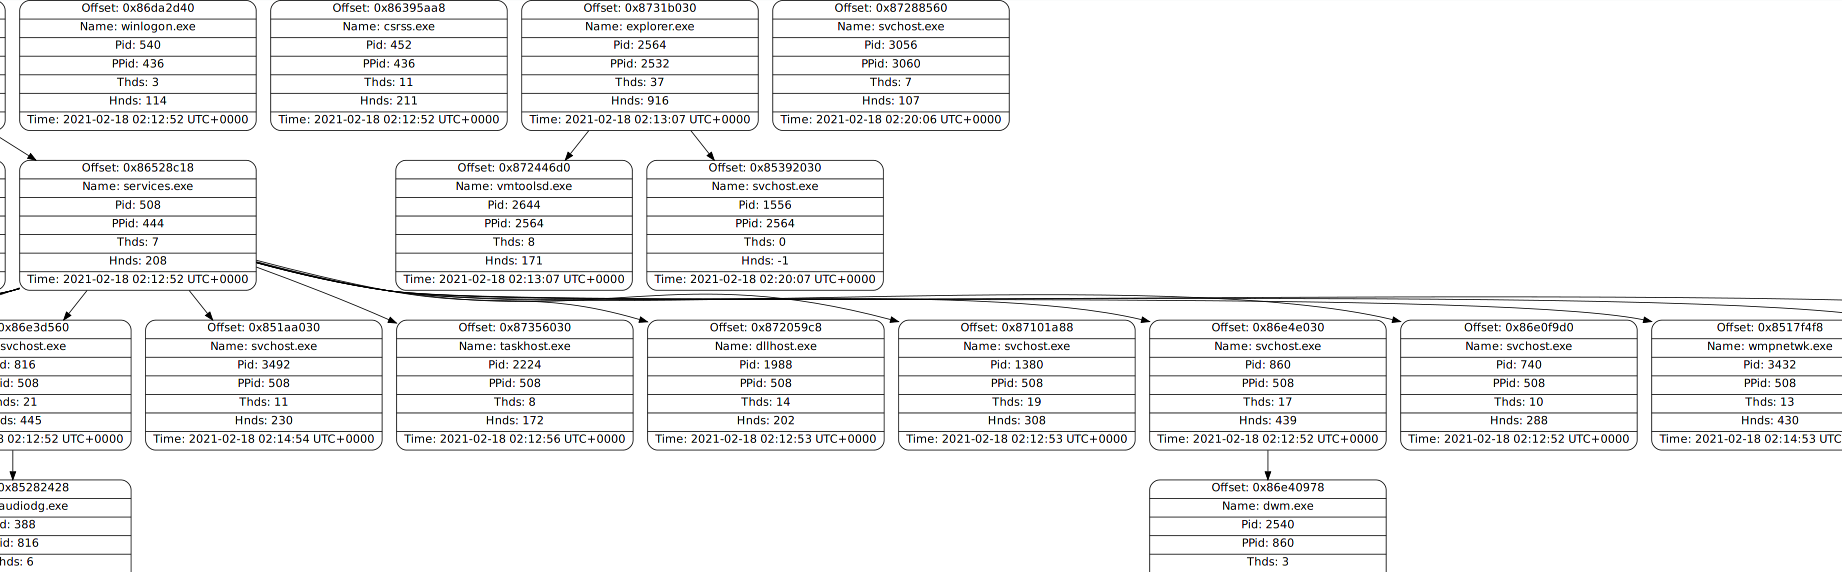
\includegraphics[width=\columnwidth]{pics/pstree.png}
						\caption{Volatility pstree: Running Process tree}
						\label{pstree}
					\end{figure}
					The process tree of the running process in the dumped memory shows \textit{svchost.exe (PID 3056, top right)}
					being spawned as disjoint from \textit{services.exe (PID 508, left)}. This, in an ordinary system is not
					possible and hence makes the process \textit{PID 3056} suspicious.

					\begin{figure}[!htbp]% [!hb] forces image to be placed at that position
						\centering
						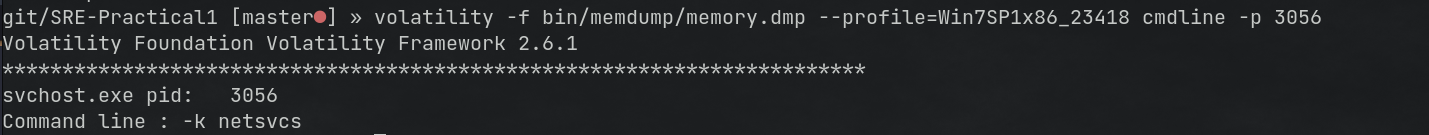
\includegraphics[width=\columnwidth]{pics/svchost_cmdline.png}
						\caption{Volatility cmdline: Commandline for the PID 3056}
						\label{svchostCmdline}
					\end{figure}
					The process \textit{PID 3056} was started with the option \textit{`-k netsvcs'} (Fig. \ref{svchostCmdline}).

					\begin{figure}[!htbp]% [!hb] forces image to be placed at that position
						\centering
						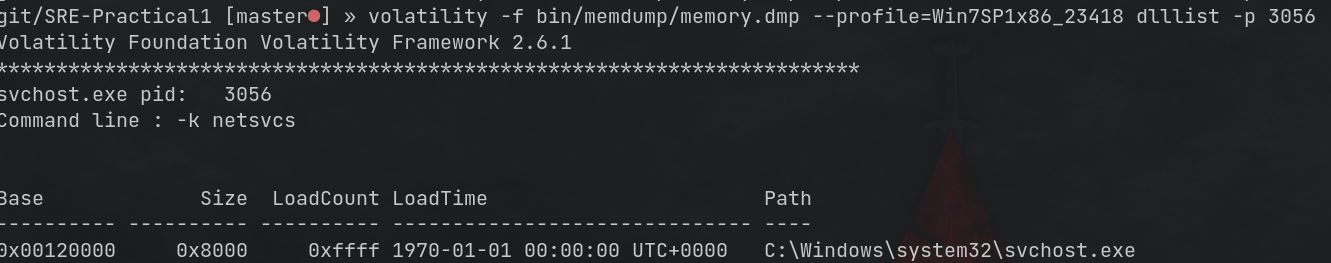
\includegraphics[width=\columnwidth]{pics/svchostPath.png}
						\caption{Volatility dlllist: Path of the executable}
						\label{svchostPath}
					\end{figure}
					Moreover, the executable path corresponds to legitimate path of the process (Fig. \ref{svchostPath}). Also, the \textit{``ldrmodules''} output is consistent with the \textit{``dlllist''} output. This asserts that none of the libraries that were loaded by this process have been maliciously replaced from their path on the file system or no new library has been loaded without the notice to userspace. 

					\begin{figure}[!htbp]% [!hb] forces image to be placed at that position
						\centering
						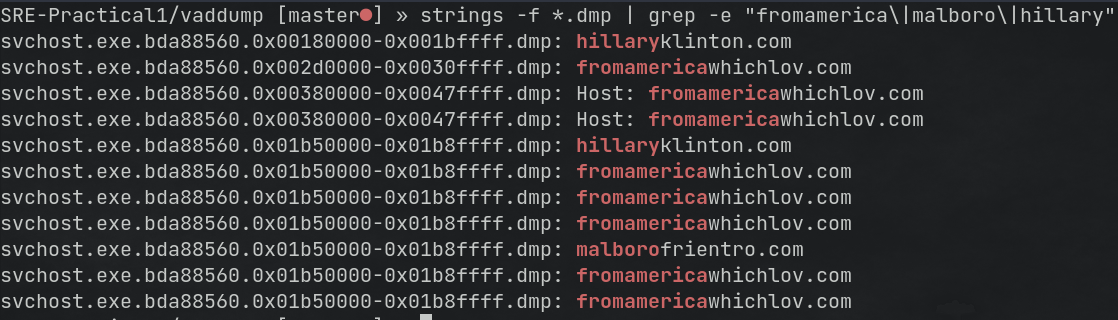
\includegraphics[width=\columnwidth]{pics/stringsdump.png}
						\caption{Volatility vaddump: Running strings on dumped VAD memory nodes}
						\label{vaddump}
					\end{figure}
					\begin{figure}[!htbp]% [!hb] forces image to be placed at that position
						\centering
						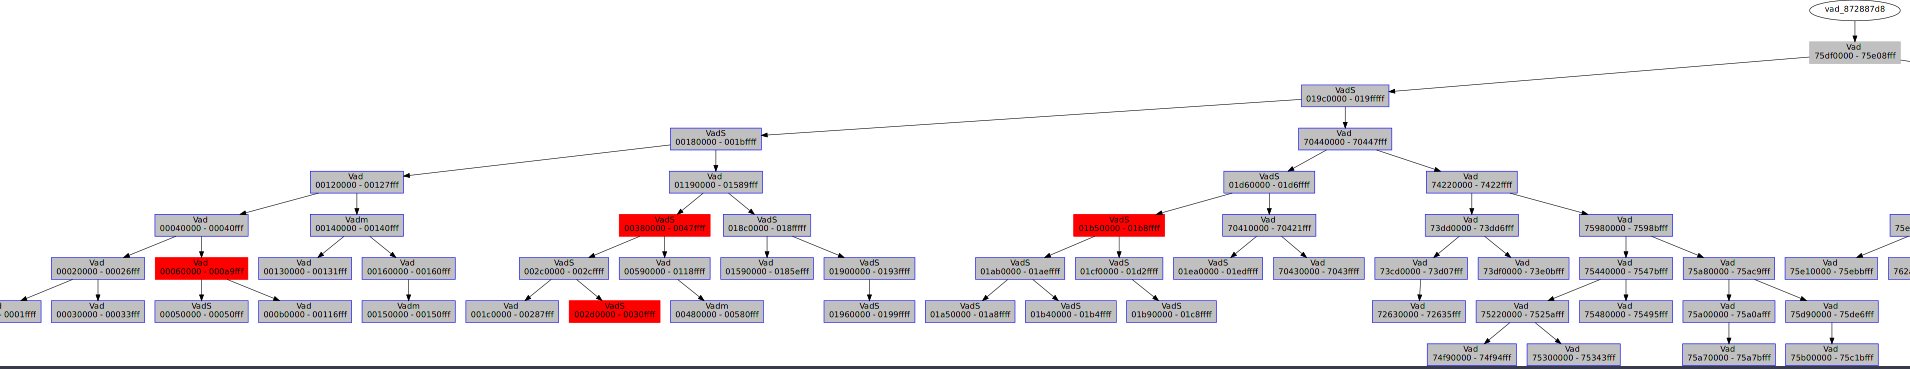
\includegraphics[width=\columnwidth]{pics/vadtree.png}
						\caption{Volatility vadtree: VAD tree of the process with malicious nodes in red}
						\label{vadtree}
					\end{figure}
					However, on dumping all the memory regions from the \textit{Virtual Address Descriptor (VAD) tree}, malicious memory regions come into view (Fig. \ref{vaddump}).
					A partial \textit{``VAD tree''} of the process \textit{``PID 3056''} is visually represented in Fig. \ref{vadtree}.

				\subsubsection{A case for Code Injection}
					\begin{figure}[!htbp]% [!hb] forces image to be placed at that position
						\centering
						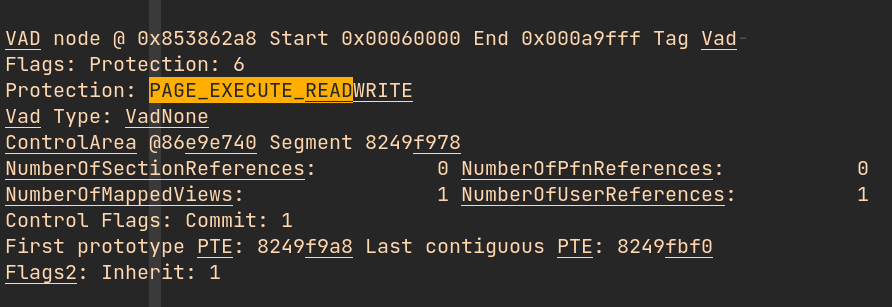
\includegraphics[width=\columnwidth]{pics/vadinfo.png}
						\caption{Volatility vadinfo: Memory section with injected code}
						\label{vadtree}
					\end{figure}
					\begin{figure}[!htbp]% [!hb] forces image to be placed at that position
						\centering
						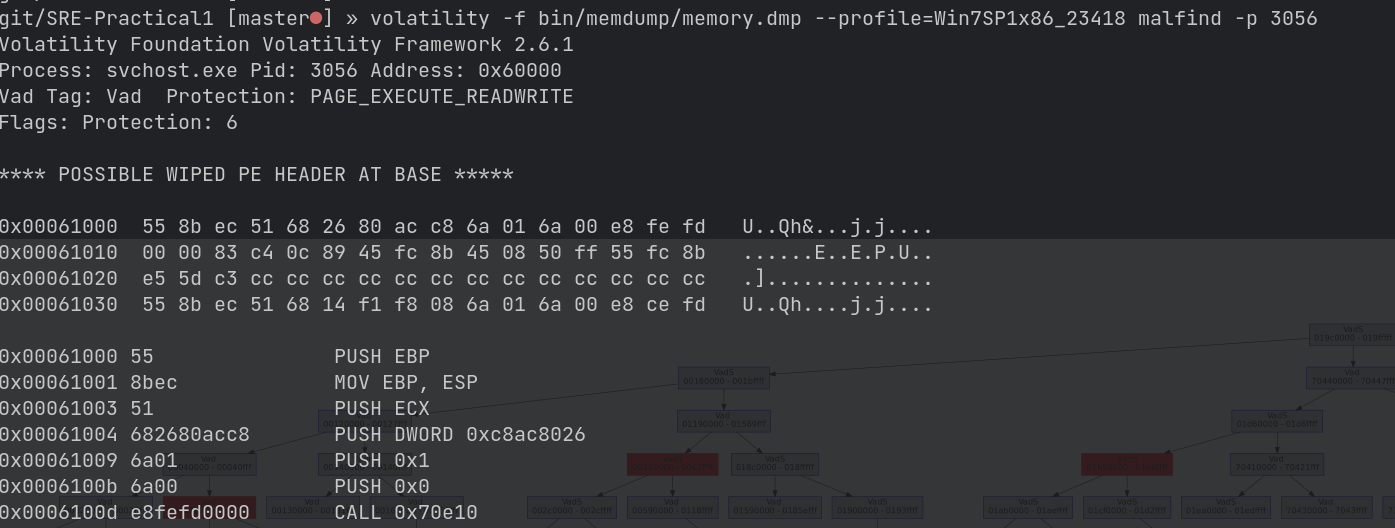
\includegraphics[width=\columnwidth]{pics/malfind.png}
						\caption{Volatility malfind: Malfind report}
						\label{malfind}
					\end{figure}
					The output to \textit{``vadinfo''} module reveals that a memory region, consistent with previous observations, has a \textit{`PAGE\_EXECUTE\_READWRITE'} permission.
					This permission and memory base combination along with a possibly wiped \textit{PE header} is also reported by \textit{`malfind'} plugin, confirming the suspicion of injected code (Fig. \ref{malfind}).

				\subsubsection{Memory region analysis}
					\begin{figure}[!htbp]% [!hb] forces image to be placed at that position
						\centering
						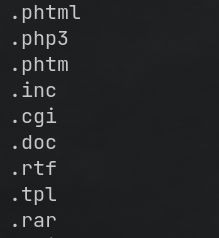
\includegraphics[width=\columnwidth]{pics/extns.png}
						\caption{The HTTP POST file extensions}
						\label{extns}
					\end{figure}
					On analyzing the memory regions, a few following features are observed (shown in Appendix A attached at the end of the report),
					\begin{itemize}
						\item Multiple string references to \textit{``bank''} and a URL confirms to a certain degree that malware is somehow associated with banking applications.
						\item Multiple string references to browser profiles and \textit{``Micromedia''} imply applications such as browsers and flash player, possibly having to do with internet User Agents.
						\item A peculiar string with reference to \textit{bot id} hints towards a BotNet like functionality.
						\item A set of extensions being found in Fig. \ref{extns} shows how many extensions can the files sent via HTTP POST have.
						\item A reference to \textit{``Java''} indicates some java related functionality.
						\item Some strings, a reference to \textit{`Keylogger.h'} and keylogger thread hint towards keylogger functionality.
					\end{itemize}
\section{Indicators of Compromise}
			\subsection{Network Based}
				The network based indicators is the connection/lookup to the following domains:
				\begin{itemize}
					\item fromamericawhichlove.com
					\item hillaryklinton.com
					\item malborofrientro.com
				\end{itemize}
			\subsection{Host Based}
				\begin{figure}[!htbp]% [!hb] forces image to be placed at that position
					\centering
					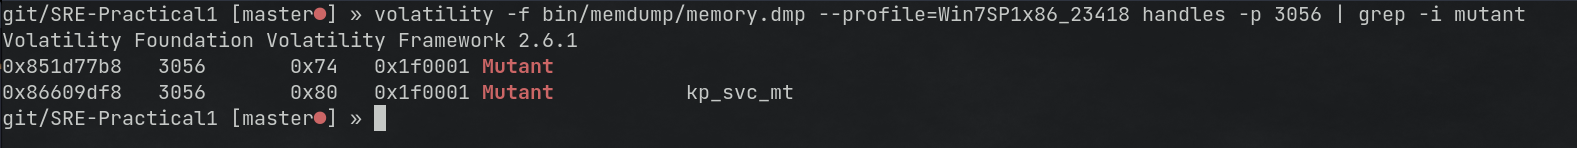
\includegraphics[width=\columnwidth]{pics/mutant.png}
					\caption{Volatility handles: Suspicious handle of PID 3056}
					\label{mutant}
				\end{figure}
				The host based indicators is the presence of the following,
				\begin{itemize}
					\item \textit{``\%USERPROFILE\%\textbackslash AppData\textbackslash Roaming\textbackslash MicroST''} directory
					\item \textit{``C:\textbackslash uN7vnXGy6vErSWw''} directory
					\item \textit{``HKU\textbackslash S-1-5-21-1715238675-2618861422-3236400253-1004\textbackslash Software\textbackslash Microsoft\textbackslash Windows\textbackslash CurrentVersion\textbackslash Explorer\textbackslash UserAssist\textbackslash\{CEBFF5CD-ACE2-4F4F-9178-9926F41749EA\}\textbackslash Count\textbackslash P:\textbackslash Hfref\textbackslash znyjner\textbackslash Qrfxgbc\textbackslash Qlanzvp Nanylfvf\textbackslash Cnpxntrf\textbackslash ErtFubg\textbackslash ertfubg.rkr''} registry key.
					\item \textit{``HKU\textbackslash S-1-5-21-1715238675-2618861422-3236400253-1004\textbackslash Software\textbackslash Microsoft\textbackslash Windows\textbackslash CurrentVersion\textbackslash Explorer\textbackslash UserAssist\textbackslash\{CEBFF5CD-ACE2-4F4F-9178-9926F41749EA\}\textbackslash Count\textbackslash P:\textbackslash Hfref\textbackslash znyjner\textbackslash Qrfxgbc\textbackslash Cenpgvpny1.rkr''} registry key.
					\item \textit{``\%USERPROFILE\%\textbackslash AppData\textbackslash Roaming\textbackslash Microsoft\textbackslash Windows\textbackslash Start Menu\textbackslash Programs\textbackslash Startup\textbackslash 4QwT85szNcI.exe''} executable file.
					\item Mutant handle named \textit{``kp\_svc\_mt''} (Fig. \ref{mutant})
				\end{itemize}

\newpage
\section{Appendix A: Memory Dump string analysis screenshots}
	\begin{figure}[!htbp]% [!hb] forces image to be placed at that position
		\centering
		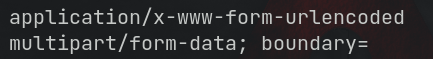
\includegraphics[width=\columnwidth]{pics/sus1.png}
	\end{figure}
	\begin{figure}[!htbp]% [!hb] forces image to be placed at that position
		\centering
		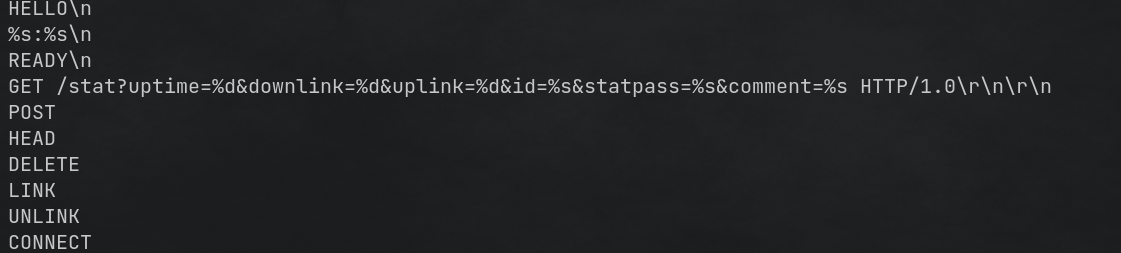
\includegraphics[width=\columnwidth]{pics/sus2.png}
	\end{figure}
	\begin{figure}[!htbp]% [!hb] forces image to be placed at that position
		\centering
		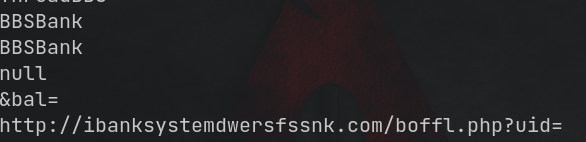
\includegraphics[width=\columnwidth]{pics/sus3.png}
	\end{figure}
	\begin{figure}[!htbp]% [!hb] forces image to be placed at that position
		\centering
		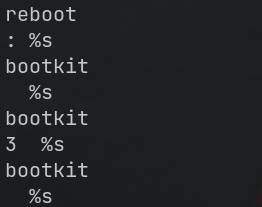
\includegraphics[width=\columnwidth]{pics/sus4.png}
	\end{figure}
	\begin{figure}[!htbp]% [!hb] forces image to be placed at that position
		\centering
		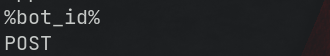
\includegraphics[width=\columnwidth]{pics/sus5.png}
	\end{figure}
	\begin{figure}[!htbp]% [!hb] forces image to be placed at that position
		\centering
		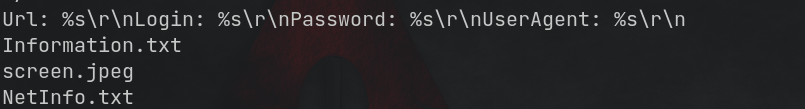
\includegraphics[width=\columnwidth]{pics/sus6.png}
	\end{figure}
	\begin{figure}[!htbp]% [!hb] forces image to be placed at that position
		\centering
		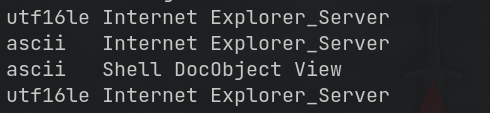
\includegraphics[width=\columnwidth]{pics/sus7.png}
	\end{figure}
	\begin{figure}[!htbp]% [!hb] forces image to be placed at that position
		\centering
		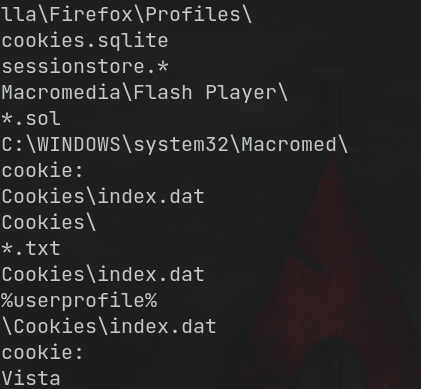
\includegraphics[width=\columnwidth]{pics/sus8.png}
	\end{figure}
	\begin{figure}[!htbp]% [!hb] forces image to be placed at that position
		\centering
		
\includegraphics[width=\columnwidth]{pics/sus9.png}
	\end{figure}
	\begin{figure}[!htbp]% [!hb] forces image to be placed at that position
		\centering
		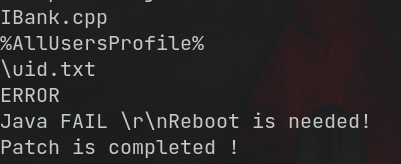
\includegraphics[width=\columnwidth]{pics/sus10.png}
	\end{figure}
	\begin{figure}[!htbp]% [!hb] forces image to be placed at that position
		\centering
		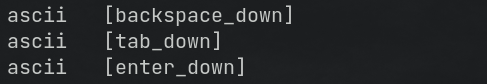
\includegraphics[width=\columnwidth]{pics/sus11.png}
	\end{figure}
	\begin{figure}[!htbp]% [!hb] forces image to be placed at that position
		\centering
		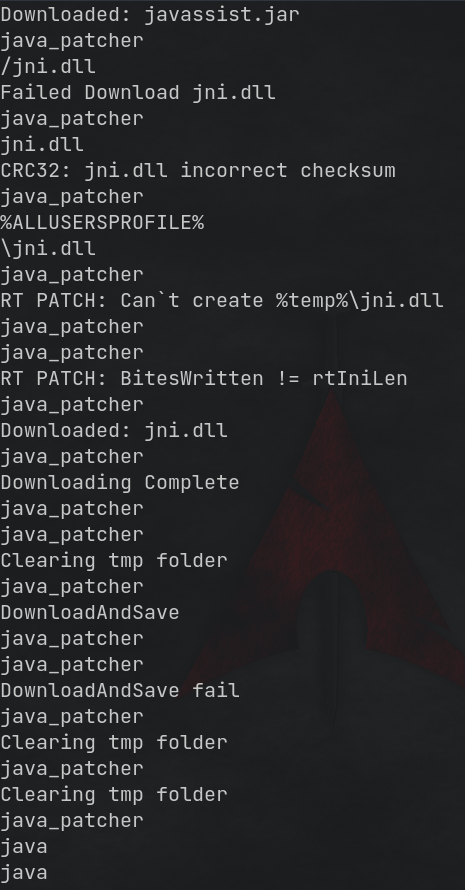
\includegraphics[width=\columnwidth]{pics/sus12.png}
	\end{figure}
	\begin{figure}[!htbp]% [!hb] forces image to be placed at that position
		\centering
		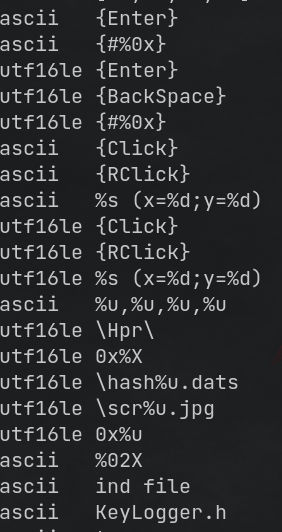
\includegraphics[width=\columnwidth]{pics/sus13.png}
	\end{figure}
	\begin{figure}[!htbp]% [!hb] forces image to be placed at that position
		\centering
		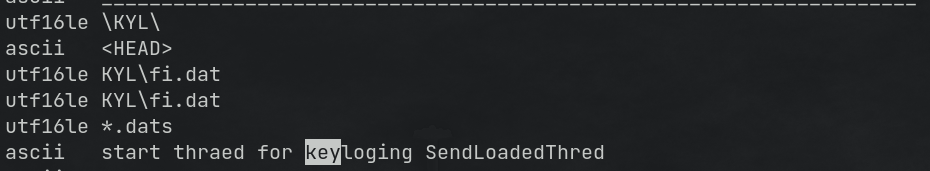
\includegraphics[width=\columnwidth]{pics/sus14.png}
	\end{figure}
	\begin{figure}[!htbp]% [!hb] forces image to be placed at that position
		\centering
		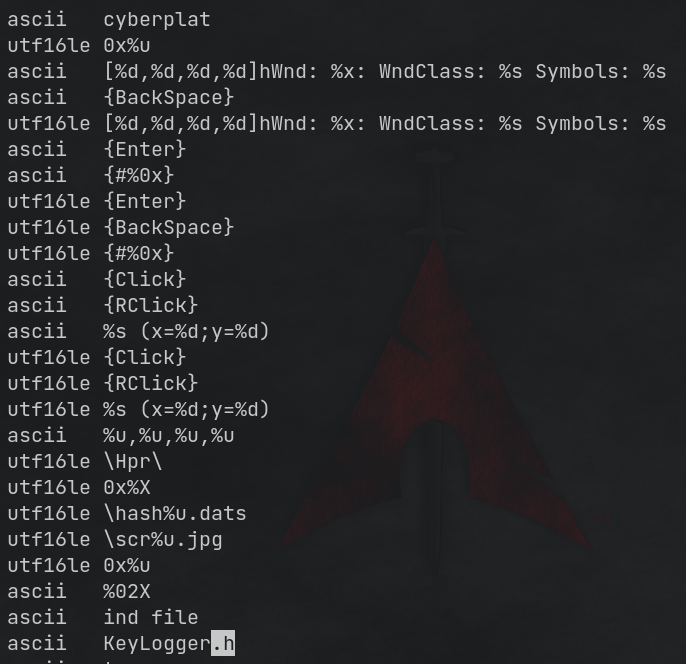
\includegraphics[width=\columnwidth]{pics/sus15.png}
	\end{figure}

\newpage
\printbibliography
\end{document}